\documentclass{article}

\usepackage[]{../../classes/dim}

\usepackage{listings}

\lstdefinelanguage{Rust}{%
  sensitive%
, morecomment=[l]{//}%
, morecomment=[s]{/*}{*/}%
, moredelim=[s][{\itshape\color[rgb]{0,0,0.75}}]{\#[}{]}%
, morestring=[b]{"}%
, alsodigit={}%
, alsoother={}%
, alsoletter={!}%
%
% 
% [1] reserve keywords
% [2] traits
% [3] primitive types
% [4] type and value constructors
% [5] identifier
%
, morekeywords={break, continue, else, for, if, in, loop, match, return, while}  % control flow keywords
, morekeywords={as, const, let, move, mut, ref, static}  % in the context of variables
, morekeywords={dyn, enum, fn, impl, Self, self, struct, trait, type, union, use, where}  % in the context of declarations
, morekeywords={crate, extern, mod, pub, super}  % in the context of modularisation
, morekeywords={unsafe}  % markers
, morekeywords={abstract, alignof, become, box, do, final, macro, offsetof, override, priv, proc, pure, sizeof, typeof, unsized, virtual, yield}  % reserved identifiers
%
% grep 'pub trait [A-Za-z][A-Za-z0-9]*' -r . | sed 's/^.*pub trait \([A-Za-z][A-Za-z0-9]*\).*/\1/g' | sort -u | tr '\n' ',' | sed 's/^\(.*\),$/{\1}\n/g' | sed 's/,/, /g'
, morekeywords=[2]{Add, AddAssign, Any, AsciiExt, AsInner, AsInnerMut, AsMut, AsRawFd, AsRawHandle, AsRawSocket, AsRef, Binary, BitAnd, BitAndAssign, Bitor, BitOr, BitOrAssign, BitXor, BitXorAssign, Borrow, BorrowMut, Boxed, BoxPlace, BufRead, BuildHasher, CastInto, CharExt, Clone, CoerceUnsized, CommandExt, Copy, Debug, DecodableFloat, Default, Deref, DerefMut, DirBuilderExt, DirEntryExt, Display, Div, DivAssign, DoubleEndedIterator, DoubleEndedSearcher, Drop, EnvKey, Eq, Error, ExactSizeIterator, ExitStatusExt, Extend, FileExt, FileTypeExt, Float, Fn, FnBox, FnMut, FnOnce, Freeze, From, FromInner, FromIterator, FromRawFd, FromRawHandle, FromRawSocket, FromStr, FullOps, FusedIterator, Generator, Hash, Hasher, Index, IndexMut, InPlace, Int, Into, IntoCow, IntoInner, IntoIterator, IntoRawFd, IntoRawHandle, IntoRawSocket, IsMinusOne, IsZero, Iterator, JoinHandleExt, LargeInt, LowerExp, LowerHex, MetadataExt, Mul, MulAssign, Neg, Not, Octal, OpenOptionsExt, Ord, OsStrExt, OsStringExt, Packet, PartialEq, PartialOrd, Pattern, PermissionsExt, Place, Placer, Pointer, Product, Put, RangeArgument, RawFloat, Read, Rem, RemAssign, Seek, Shl, ShlAssign, Shr, ShrAssign, Sized, SliceConcatExt, SliceExt, SliceIndex, Stats, Step, StrExt, Sub, SubAssign, Sum, Sync, TDynBenchFn, Terminal, Termination, ToOwned, ToSocketAddrs, ToString, Try, TryFrom, TryInto, UnicodeStr, Unsize, UpperExp, UpperHex, WideInt, Write}
, morekeywords=[2]{Send}  % additional traits
%
, morekeywords=[3]{bool, char, f32, f64, i8, i16, i32, i64, isize, str, u8, u16, u32, u64, unit, usize, i128, u128}  % primitive types
%
, morekeywords=[4]{Err, false, None, Ok, Some, true}  % prelude value constructors
% grep 'pub \(type\|struct\|enum\) [A-Za-z][A-Za-z0-9]*' -r . | sed 's/^.*pub \(type\|struct\|enum\) \([A-Za-z][A-Za-z0-9]*\).*/\2/g' | sort -u | tr '\n' ',' | sed 's/^\(.*\),$/{\1}\n/g' | sed 's/,/, /g'    
, morekeywords=[3]{AccessError, Adddf3, AddI128, AddoI128, AddoU128, ADDRESS, ADDRESS64, addrinfo, ADDRINFOA, AddrParseError, Addsf3, AddU128, advice, aiocb, Alignment, AllocErr, AnonPipe, Answer, Arc, Args, ArgsInnerDebug, ArgsOs, Argument, Arguments, ArgumentV1, Ashldi3, Ashlti3, Ashrdi3, Ashrti3, AssertParamIsClone, AssertParamIsCopy, AssertParamIsEq, AssertUnwindSafe, AtomicBool, AtomicPtr, Attr, auxtype, auxv, BackPlace, BacktraceContext, Barrier, BarrierWaitResult, Bencher, BenchMode, BenchSamples, BinaryHeap, BinaryHeapPlace, blkcnt, blkcnt64, blksize, BOOL, boolean, BOOLEAN, BoolTrie, BorrowError, BorrowMutError, Bound, Box, bpf, BTreeMap, BTreeSet, Bucket, BucketState, Buf, BufReader, BufWriter, Builder, BuildHasherDefault, BY, BYTE, Bytes, CannotReallocInPlace, cc, Cell, Chain, CHAR, CharIndices, CharPredicateSearcher, Chars, CharSearcher, CharsError, CharSliceSearcher, CharTryFromError, Child, ChildPipes, ChildStderr, ChildStdin, ChildStdio, ChildStdout, Chunks, ChunksMut, ciovec, clock, clockid, Cloned, cmsgcred, cmsghdr, CodePoint, Color, ColorConfig, Command, CommandEnv, Component, Components, CONDITION, condvar, Condvar, CONSOLE, CONTEXT, Count, Cow, cpu, CRITICAL, CStr, CString, CStringArray, Cursor, Cycle, CycleIter, daddr, DebugList, DebugMap, DebugSet, DebugStruct, DebugTuple, Decimal, Decoded, DecodeUtf16, DecodeUtf16Error, DecodeUtf8, DefaultEnvKey, DefaultHasher, dev, device, Difference, Digit32, DIR, DirBuilder, dircookie, dirent, dirent64, DirEntry, Discriminant, DISPATCHER, Display, Divdf3, Divdi3, Divmoddi4, Divmodsi4, Divsf3, Divsi3, Divti3, dl, Dl, Dlmalloc, Dns, DnsAnswer, DnsQuery, dqblk, Drain, DrainFilter, Dtor, Duration, DwarfReader, DWORD, DWORDLONG, DynamicLibrary, Edge, EHAction, EHContext, Elf32, Elf64, Empty, EmptyBucket, EncodeUtf16, EncodeWide, Entry, EntryPlace, Enumerate, Env, epoll, errno, Error, ErrorKind, EscapeDebug, EscapeDefault, EscapeUnicode, event, Event, eventrwflags, eventtype, ExactChunks, ExactChunksMut, EXCEPTION, Excess, ExchangeHeapSingleton, exit, exitcode, ExitStatus, Failure, fd, fdflags, fdsflags, fdstat, ff, fflags, File, FILE, FileAttr, filedelta, FileDesc, FilePermissions, filesize, filestat, FILETIME, filetype, FileType, Filter, FilterMap, Fixdfdi, Fixdfsi, Fixdfti, Fixsfdi, Fixsfsi, Fixsfti, Fixunsdfdi, Fixunsdfsi, Fixunsdfti, Fixunssfdi, Fixunssfsi, Fixunssfti, Flag, FlatMap, Floatdidf, FLOATING, Floatsidf, Floatsisf, Floattidf, Floattisf, Floatundidf, Floatunsidf, Floatunsisf, Floatuntidf, Floatuntisf, flock, ForceResult, FormatSpec, Formatted, Formatter, Fp, FpCategory, fpos, fpos64, fpreg, fpregset, FPUControlWord, Frame, FromBytesWithNulError, FromUtf16Error, FromUtf8Error, FrontPlace, fsblkcnt, fsfilcnt, fsflags, fsid, fstore, fsword, FullBucket, FullBucketMut, FullDecoded, Fuse, GapThenFull, GeneratorState, gid, glob, glob64, GlobalDlmalloc, greg, group, GROUP, Guard, GUID, Handle, HANDLE, Handler, HashMap, HashSet, Heap, HINSTANCE, HMODULE, hostent, HRESULT, id, idtype, if, ifaddrs, IMAGEHLP, Immut, in, in6, Incoming, Infallible, Initializer, ino, ino64, inode, input, InsertResult, Inspect, Instant, int16, int32, int64, int8, integer, IntermediateBox, Internal, Intersection, intmax, IntoInnerError, IntoIter, IntoStringError, intptr, InvalidSequence, iovec, ip, IpAddr, ipc, Ipv4Addr, ipv6, Ipv6Addr, Ipv6MulticastScope, Iter, IterMut, itimerspec, itimerval, jail, JoinHandle, JoinPathsError, KDHELP64, kevent, kevent64, key, Key, Keys, KV, l4, LARGE, lastlog, launchpad, Layout, Lazy, lconv, Leaf, LeafOrInternal, Lines, LinesAny, LineWriter, linger, linkcount, LinkedList, load, locale, LocalKey, LocalKeyState, Location, lock, LockResult, loff, LONG, lookup, lookupflags, LookupHost, LPBOOL, LPBY, LPBYTE, LPCSTR, LPCVOID, LPCWSTR, LPDWORD, LPFILETIME, LPHANDLE, LPOVERLAPPED, LPPROCESS, LPPROGRESS, LPSECURITY, LPSTARTUPINFO, LPSTR, LPVOID, LPWCH, LPWIN32, LPWSADATA, LPWSAPROTOCOL, LPWSTR, Lshrdi3, Lshrti3, lwpid, M128A, mach, major, Map, mcontext, Metadata, Metric, MetricMap, mflags, minor, mmsghdr, Moddi3, mode, Modsi3, Modti3, MonitorMsg, MOUNT, mprot, mq, mqd, msflags, msghdr, msginfo, msglen, msgqnum, msqid, Muldf3, Mulodi4, Mulosi4, Muloti4, Mulsf3, Multi3, Mut, Mutex, MutexGuard, MyCollection, n16, NamePadding, NativeLibBoilerplate, nfds, nl, nlink, NodeRef, NoneError, NonNull, NonZero, nthreads, NulError, OccupiedEntry, off, off64, oflags, Once, OnceState, OpenOptions, Option, Options, OptRes, Ordering, OsStr, OsString, Output, OVERLAPPED, Owned, Packet, PanicInfo, Param, ParseBoolError, ParseCharError, ParseError, ParseFloatError, ParseIntError, ParseResult, Part, passwd, Path, PathBuf, PCONDITION, PCONSOLE, Peekable, PeekMut, Permissions, PhantomData, pid, Pipes, PlaceBack, PlaceFront, PLARGE, PoisonError, pollfd, PopResult, port, Position, Powidf2, Powisf2, Prefix, PrefixComponent, PrintFormat, proc, Process, PROCESS, processentry, protoent, PSRWLOCK, pthread, ptr, ptrdiff, PVECTORED, Queue, radvisory, RandomState, Range, RangeFrom, RangeFull, RangeInclusive, RangeMut, RangeTo, RangeToInclusive, RawBucket, RawFd, RawHandle, RawPthread, RawSocket, RawTable, RawVec, Rc, ReadDir, Receiver, recv, RecvError, RecvTimeoutError, ReentrantMutex, ReentrantMutexGuard, Ref, RefCell, RefMut, REPARSE, Repeat, Result, Rev, Reverse, riflags, rights, rlim, rlim64, rlimit, rlimit64, roflags, Root, RSplit, RSplitMut, RSplitN, RSplitNMut, RUNTIME, rusage, RwLock, RWLock, RwLockReadGuard, RwLockWriteGuard, sa, SafeHash, Scan, sched, scope, sdflags, SearchResult, SearchStep, SECURITY, SeekFrom, segment, Select, SelectionResult, sem, sembuf, send, Sender, SendError, servent, sf, Shared, shmatt, shmid, ShortReader, ShouldPanic, Shutdown, siflags, sigaction, SigAction, sigevent, sighandler, siginfo, Sign, signal, signalfd, SignalToken, sigset, sigval, Sink, SipHasher, SipHasher13, SipHasher24, size, SIZE, Skip, SkipWhile, Slice, SmallBoolTrie, sockaddr, SOCKADDR, sockcred, Socket, SOCKET, SocketAddr, SocketAddrV4, SocketAddrV6, socklen, speed, Splice, Split, SplitMut, SplitN, SplitNMut, SplitPaths, SplitWhitespace, spwd, SRWLOCK, ssize, stack, STACKFRAME64, StartResult, STARTUPINFO, stat, Stat, stat64, statfs, statfs64, StaticKey, statvfs, StatVfs, statvfs64, Stderr, StderrLock, StderrTerminal, Stdin, StdinLock, Stdio, StdioPipes, Stdout, StdoutLock, StdoutTerminal, StepBy, String, StripPrefixError, StrSearcher, subclockflags, Subdf3, SubI128, SuboI128, SuboU128, subrwflags, subscription, Subsf3, SubU128, Summary, suseconds, SYMBOL, SYMBOLIC, SymmetricDifference, SyncSender, sysinfo, System, SystemTime, SystemTimeError, Take, TakeWhile, tcb, tcflag, TcpListener, TcpStream, TempDir, TermInfo, TerminfoTerminal, termios, termios2, TestDesc, TestDescAndFn, TestEvent, TestFn, TestName, TestOpts, TestResult, Thread, threadattr, threadentry, ThreadId, tid, time, time64, timespec, TimeSpec, timestamp, timeval, timeval32, timezone, tm, tms, ToLowercase, ToUppercase, TraitObject, TryFromIntError, TryFromSliceError, TryIter, TryLockError, TryLockResult, TryRecvError, TrySendError, TypeId, U64x2, ucontext, ucred, Udivdi3, Udivmoddi4, Udivmodsi4, Udivmodti4, Udivsi3, Udivti3, UdpSocket, uid, UINT, uint16, uint32, uint64, uint8, uintmax, uintptr, ulflags, ULONG, ULONGLONG, Umoddi3, Umodsi3, Umodti3, UnicodeVersion, Union, Unique, UnixDatagram, UnixListener, UnixStream, Unpacked, UnsafeCell, UNWIND, UpgradeResult, useconds, user, userdata, USHORT, Utf16Encoder, Utf8Error, Utf8Lossy, Utf8LossyChunk, Utf8LossyChunksIter, utimbuf, utmp, utmpx, utsname, uuid, VacantEntry, Values, ValuesMut, VarError, Variables, Vars, VarsOs, Vec, VecDeque, vm, Void, WaitTimeoutResult, WaitToken, wchar, WCHAR, Weak, whence, WIN32, WinConsole, Windows, WindowsEnvKey, winsize, WORD, Wrapping, wrlen, WSADATA, WSAPROTOCOL, WSAPROTOCOLCHAIN, Wtf8, Wtf8Buf, Wtf8CodePoints, xsw, xucred, Zip, zx}
%
, morekeywords=[5]{assert!, assert_eq!, assert_ne!, cfg!, column!, compile_error!, concat!, concat_idents!, debug_assert!, debug_assert_eq!, debug_assert_ne!, env!, eprint!, eprintln!, file!, format!, format_args!, include!, include_bytes!, include_str!, line!, module_path!, option_env!, panic!, print!, println!, select!, stringify!, thread_local!, try!, unimplemented!, unreachable!, vec!, write!, writeln!}  % prelude macros
}%

\lstdefinestyle{colouredRust}%
{ basicstyle=\ttfamily%
, identifierstyle=%
, commentstyle=\color[gray]{0.4}%
, stringstyle=\color[rgb]{b}%
, keywordstyle=\bfseries% reserved keywords
, keywordstyle=[2]\color{r}% traits
, keywordstyle=[4]\color{g}% primitive types
, keywordstyle=[3]\color{g}% type and value constructors
, keywordstyle=[1]\color{b}% macros
, columns=spaceflexible%
, keepspaces=true%
, showspaces=false%
, showtabs=false%
, showstringspaces=true%
}%

\lstset{style=colouredRust}

\usepackage{float}
\usepackage{tikz}
\usetikzlibrary {automata,positioning}
\usepackage{multicol}

\begin{document}
    \header{Homework}
    {Algorithms and Data Structures}

    \begin{center}
        \large
        Worksheet 8
    \end{center}
    \begin{tasks}
        \item {
            \begin{enumerate}
                \item {\
                    \begin{figure}[H]
                        \centering
                        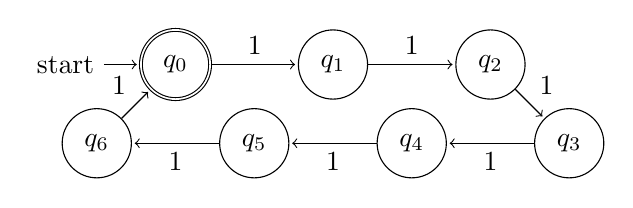
\begin{tikzpicture}[shorten >=1pt,node distance=2cm,on grid,auto]
                            % \draw[help lines] (-2,0) grid (4,-5);

                            \node[state,initial,accepting]  (q_0)                {$q_0$};
                            \node[state]          (q_1) [right=of q_0] {$q_1$};
                            \node[state]          (q_2) [right=of q_1] {$q_2$};
                            \node[state]          (q_3) at (5, -1) {$q_3$};
                            \node[state]          (q_4) [left=of q_3] {$q_4$};
                            \node[state]          (q_5) [left=of q_4] {$q_5$};
                            \node[state]          (q_6) [left=of q_5] {$q_6$};
                            % \node[state]          (end) at (1, -2.4) {end};
                            
                            \path[->] 
                                (q_0)   edge [] node   {1} (q_1)
                                        % edge [loop above] node  {0} (end)
                                (q_1)   edge [] node   {1} (q_2)
                                        % edge [] node            {0} (end)
                                (q_2)   edge [] node   {1} (q_3)
                                        % edge [] node  [] {0} (end)
                                (q_3)   edge [] node   {1} (q_4)
                                        % edge [] node [] {0} (end)
                                (q_4)   edge [] node   {1} (q_5)
                                        % edge [] node []{0} (end)
                                (q_5)   edge [] node   {1} (q_6)
                                        % edge [] node   {0} (end)
                                (q_6)   edge [] node   {1} (q_0)
                                        % edge [] node   {0} (end)
                                        ;
                        \end{tikzpicture}
                    \end{figure}
                }
                \item {\
                    \begin{figure}[H]
                        \centering
                        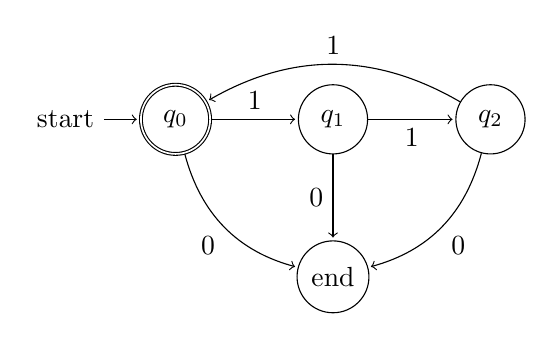
\begin{tikzpicture}[shorten >=1pt,node distance=2cm,on grid,auto]
                            % \draw[help lines] (-1,0) grid (5,-4);

                            \node[state,initial,accepting]  (q_0)                {$q_0$};
                            \node[state]          (q_1) [right=of q_0] {$q_1$};
                            \node[state]          (end) [below=of q_1] {end};
                            \node[state]          (q_2) [right=of q_1] {$q_2$};
                            
                            \path[->] 
                                (q_0)   edge [] node [] {1} (q_1)
                                        edge [bend right] node [swap] {0} (end)
                                (q_1)   edge [] node [swap] {1} (q_2)
                                        edge [] node [swap] {0} (end)
                                (q_2)   edge [bend right] node [swap] {1} (q_0)
                                        edge [bend left] node [] {0} (end);
                        \end{tikzpicture}
                    \end{figure}
                }
            \end{enumerate}
        }
        \item {
            \begin{enumerate}
                \item \begin{displaymath}
                    \begin{aligned}
                        f(1) &= 0, & f(2) &= 0,\\ 
                        f(3) &= 1, & f(4) &= 2,\\ 
                        f(5) &= 3, & f(6) &= 4
                    \end{aligned}
                \end{displaymath}
                \item {\
                    \begin{figure}[H]
                        \centering
                        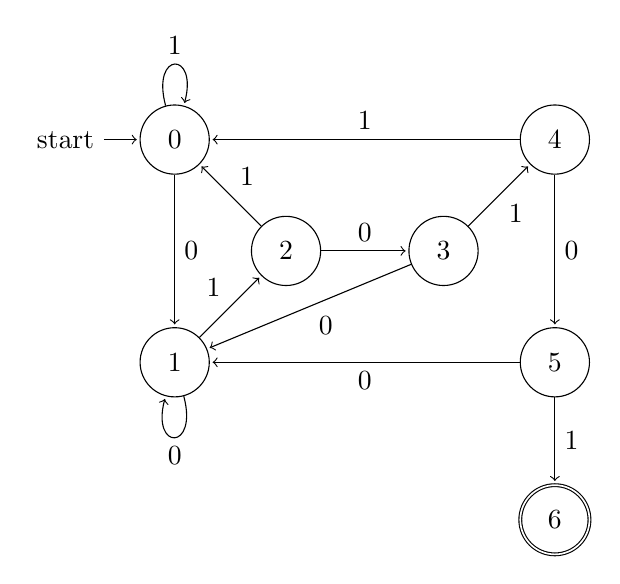
\begin{tikzpicture}[shorten >=1pt,node distance=2cm,on grid,auto]
                            \node[state,initial]  (0)   {$0$};
                            \node[state]          (2) [below right=of 0]   {$2$};
                            \node[state]          (3) [right=of 2]   {$3$};
                            \node[state]          (4) [above right=of 3]  {$4$};
                            \node[state]          (5) [below right=of 3] {$5$};
                            \node[state]          (1) [below left=of 2]   {$1$};
                            \node[state,accepting](6) [below=of 5] {$6$};
                            
                            \path[->] 
                                (0) edge node {0} (1)
                                    edge [loop above] node {1} (0)
                                (1) edge node {1} (2)
                                    edge [loop below] node {0} (1)
                                (2) edge node {0} (3)
                                    edge node [swap] {1} (0)
                                (3) edge node [swap] {1} (4)
                                    edge node {0} (1)
                                (4) edge node {0} (5)
                                    edge node [swap] {1} (0)
                                (5) edge node {0} (1)
                                    edge node {1} (6);
                        \end{tikzpicture}
                    \end{figure}
                }
                \item \begin{displaymath}
                    \begin{aligned}
                        f(1) &= 0, & f(2) &= 0, \\
                        f(3) &= 1, & f(4) &= 2, \\
                        f(5) &= 0, & f(6) &= 0, \\
                        f(7) &= 1, & f(8) &= 2 \\
                    \end{aligned}
                \end{displaymath}
                \item {\
                \begin{figure}[H]
                    \centering
                    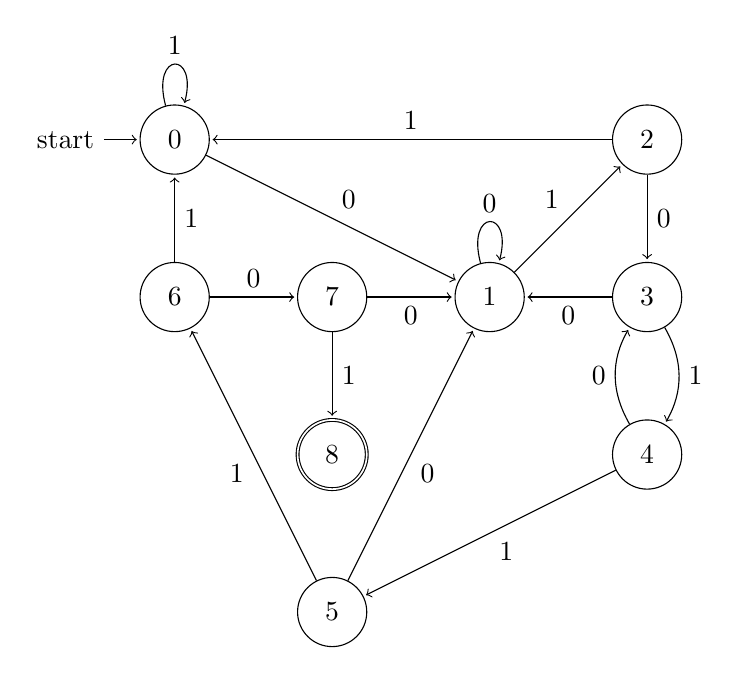
\begin{tikzpicture}[shorten >=1pt,node distance=2cm,on grid,auto]
                        % \draw[help lines] (-1,0) grid (5,-4);

                        \node[state,initial]  (0) at (0, 0)     {$0$};
                        \node[state]          (6) [below=of 0]  {$6$};
                        \node[state]          (7) [right=of 6]  {$7$};
                        \node[state]          (1) [right=of 7]  {$1$};
                        \node[state]          (3) [right=of 1]  {$3$};
                        \node[state]          (2) [above=of 3]  {$2$};
                        \node[state,accepting](8) [below=of 7]  {$8$};
                        \node[state]          (5) [below=of 8]  {$5$};
                        \node[state]          (4) [below=of 3]  {$4$};
                        
                        \path[->] 
                            (0) edge node {0} (1)
                                edge [loop above] node {1} (0)
                            (1) edge node {1} (2)
                                edge [loop above] node {0} (1)
                            (2) edge node {0} (3)
                                edge node [swap] {1} (0)
                            (3) edge [bend left] node {1} (4)
                                edge node {0} (1)
                            (4) edge [bend left] node {0} (3)
                                edge node {1} (5)
                            (5) edge node [swap] {0} (1)
                                edge node {1} (6)
                            (6) edge node {0} (7)
                                edge node [swap] {1} (0)
                            (7) edge node [swap] {0} (1)
                                edge node {1} (8);
                    \end{tikzpicture}
                \end{figure}
            }
            \end{enumerate}
        } 
        \item \begin{lstlisting}[language=rust]
fn find_pattern(s: Vec<char>, p: Vec<char>, f: Vec<usize>) -> Option<usize> {
    let mut i = 0;
    let mut m = 0;
    while i < s.len() {
        if i - m == p.len() {
            return Some(m);
        }

        while s[i] != p[i - m] && i != m {
            m = i - f[i - m] + 1;
        }

        i += 1;
    }

    None
}
        \end{lstlisting}
    \end{tasks}
\end{document}